\documentclass[10pt]{article}
%%%%%%%%%%%%%%%%%%%%%%%%%%%%%%%%%%%%%%%%
\usepackage{amsmath}
\usepackage{verbatim}
\usepackage[usenames,dvipsnames]{color}
\usepackage{ulem}
\usepackage{setspace}
\usepackage{lscape}
\usepackage{longtable}
\usepackage[top=1.25in,bottom=1.5in,left=1in,right=1.5in,landscape]{geometry}
\usepackage{graphicx}
\usepackage{epstopdf}
\usepackage[usenames,dvipsnames]{pstricks}
\usepackage{epsfig}
\usepackage{pstricks-add}
\usepackage{pst-node}
\usepackage{fancyhdr}
\usepackage[absolute,showboxes]{textpos}

%TCIDATA{OutputFilter=LATEX.DLL}
%TCIDATA{Version=5.00.0.2552}
%TCIDATA{<META NAME="SaveForMode" CONTENT="1">}
%TCIDATA{Created=Thursday, August 28, 2003 13:38:44}
%TCIDATA{LastRevised=Thursday, August 14, 2008 15:20:27}
%TCIDATA{<META NAME="GraphicsSave" CONTENT="32">}
%TCIDATA{<META NAME="DocumentShell" CONTENT="Standard LaTeX\Blank - Standard LaTeX Article">}
%TCIDATA{Language=American English}
%TCIDATA{CSTFile=LaTeX article (bright).cst}

\setcounter{MaxMatrixCols}{10}

\newenvironment{proof}[1][Proof]{\noindent\textbf{#1.} }{\ \rule{0.5em}{0.5em}}
\setlength{\columnsep}{.2in}

\renewcommand{\labelitemii}{$\cdot$}

\pagestyle{fancy} \fancyhead{} \fancyfoot{} \rfoot{} \lfoot{}

\newcommand{\slide}[2]{
\begin{textblock}{11}(0,0)
\textcolor{Black}{\textbf{\huge \rule{0pt}{1in} \raisebox{.2in}{#1}}}
\end{textblock}
\begin{Large} \noindent
#2
\end{Large}
\vfill \pagebreak}

\setlength{\TPHorizModule}{1in}
\setlength{\TPVertModule}{1in}
\textblockcolour{Yellow}
\renewcommand{\headrulewidth}{0pt}



\begin{document}
\onehalfspacing 

\lfoot{Natural Resources} \rfoot{Economic Growth}

\slide{Resources and Growth}{Types of natural resources
\begin{itemize}
	\item Renewable: land, trees. Can think of them as a constant stock. Know that presence will slow down steady state growth
	\item Non-renewable: oil, copper, iron. Will eventually run out. How do these alter steady state growth?
\end{itemize}

\vspace{.25in}\noindent Let output be
\begin{equation}
Y = B K^{\alpha} E^{\gamma} L^{1-\alpha-\gamma}
\end{equation}
where $E$ is energy used in production. Other aspects of model will be typical
\begin{eqnarray}
\frac{\dot{B}}{B} &=& g \\
\frac{\dot{L}}{L} &=& n \\
\dot{K} &=& sY - \delta K
\end{eqnarray}
}

\slide{Resources}{Let $R_0$ be the initial stock of the non-renewable resource. With $E$ used in production at any given time, we have
\begin{equation}
\dot{R} = - E
\end{equation}

\vspace{.25in}\noindent What is $E$? Let's assume that at any given moment, we consume a fixed fraction of the remaining stock of resources, so
\begin{equation}
E = s_E R
\end{equation}
Turns out this is the result if we think about optimal models of resource use. So we'll stick with constant $s_E$.

\vspace{.25in}\noindent Combined with top equation we have
\begin{equation}
\frac{\dot{R}}{R} = - s_E.
\end{equation}
}

\slide{Evoluion of Resources}{Given $\dot{R}/R = -s_E$ is a differential equation we could solve for the following
\begin{equation}
R(t) = R_0 e^{-s_E t}
\end{equation}
and therefore
\begin{equation}
E(t) = s_E R_0 e^{-s_E t}.
\end{equation}
This equation implies (take logs and derivatives) that
\begin{equation}
\frac{\dot{E}}{E} = - s_E
\end{equation}
which implies that the amount of energy is declining constantly over time. 

\vspace{.25in}\noindent Note also that $s_E$ has two effects on the amount of energy we use. The higher is $s_E$, the more of the resource we use right now, so $E$ is higher. But the higher is $s_E$, the smaller the resource base left, so $E$ will be lower over time. 
}

\slide{Balanced Growth Path}{Again, we want to find a BGP where output per worker grows at a constant rate, and all the terms in the production function grow at constant rates as well.

\vspace{.25in}\noindent A little difficult given the $E$, so different strategy. With $Y = B K^{\alpha} E^{\gamma} L^{1-\alpha-\gamma}$ divide both side by $Y^{\alpha}$ to get
\begin{equation}
Y^{1-\alpha} = B \left( \frac{K}{Y}\right)^{\alpha} E^{\gamma} L^{1-\alpha-\gamma}
\end{equation}
and then take both sides to $1/(1-\alpha)$ to get
\begin{equation}
Y = B^{1/(1-\alpha)} \left( \frac{K}{Y}\right)^{\alpha/(1-\alpha)} E^{\gamma/(1-\alpha)} L^{(1-\alpha-\gamma)/(1-\alpha)}
\end{equation}
and in per-worker terms we have
\begin{equation}
y = B^{1/(1-\alpha)} \left( \frac{K}{Y}\right)^{\alpha/(1-\alpha)} E^{\gamma/(1-\alpha)} L^{\gamma/(1-\alpha)}
\end{equation}
}

\slide{Solving for BGP}{Given
\begin{equation}
y = B^{1/(1-\alpha)} \left( \frac{K}{Y}\right)^{\alpha/(1-\alpha)} E^{\gamma/(1-\alpha)} L^{\gamma/(1-\alpha)}
\end{equation}
we can plug in what we know about $E$ to get
\begin{equation}
y = B^{1/(1-\alpha)} \left( \frac{K}{Y}\right)^{\alpha/(1-\alpha)} \left(s_E R_0 e^{-s_E t}\right)^{\gamma/(1-\alpha)} L^{\gamma/(1-\alpha)}.
\end{equation}
Now, take logs and derivatives to find
\begin{equation}
\frac{\dot{y}}{y} = \frac{1}{1-\alpha}\frac{\dot{B}}{B} + \frac{\gamma}{1-\alpha} \frac{\dot{E}}{E} - \frac{\gamma}{1-\alpha} \frac{\dot{L}}{L} 
\end{equation}
which accounts for the fact that along the BGP $K/Y$ will be unchanging. 
}

\slide{Growth along the BGP}{Using
\begin{equation}
\frac{\dot{y}}{y} = \frac{1}{1-\alpha}\frac{\dot{B}}{B} - \frac{\gamma}{1-\alpha} \frac{\dot{E}}{E} - \frac{\gamma}{1-\alpha} \frac{\dot{L}}{L} 
\end{equation}
and what we already know we have that
\begin{equation}
g_y^{BGP} = \frac{1}{1-\alpha}g - \frac{\gamma}{1-\alpha} s_E - \frac{\gamma}{1-\alpha} n
\end{equation}
or
\begin{equation}
g_y^{BGP} = \frac{1}{1-\alpha}\left(g - \gamma (s_E+n)  \right)
\end{equation}

\vspace{.25in}\noindent So having non-renewables in acts something like the Malthusian model. We have
\begin{itemize}
	\item Slower growth due to $n$. With a fixed resource, population growth puts a drag on growth in output per worker
	\item Because the resource is winding down, we have an additional drag on growth due to $s_E$
	\item Growth in $y$ is positive only if $g > s_E +n$, or technological change is sufficiently fast.
\end{itemize}
}

\slide{Drag Effect}{How large is the drag on growth from resources? First, let's allow for land as well,
\begin{equation}
Y = B K^{\alpha} X^{\beta} E^{\gamma} L^{1-\alpha-\beta-\gamma}
\end{equation}
and $X$ does not change over time. Solving this looks identical to what we did, but with $\beta$ term carried through,
\begin{equation}
g_y^{BGP} = \frac{1}{1-\alpha}\left(g - \gamma s_E - (\beta+\gamma)n  \right)
\end{equation}
and $n$ has an additional negative effect due to land.
}


\slide{Drag Effect}{So what are these values? Nordhaus (1992) finds
\begin{itemize}
	\item $\beta = 0.1$, $\gamma = 0.1$, and $\alpha = 0.2$
	\item $n = 0.01$
	\item $s_E = 0.005$, or we are using 1/2 of 1\% of resources every year
	\item No, $s_E$ probably isn't higher today. New discoveries of many resources mean that $R_0$ is actually going up.
\end{itemize}

\vspace{.25in}\noindent The drag term 
\begin{equation}
\frac{1}{1-\alpha}\left(\gamma s_E - (\beta+\gamma)n \right) = \frac{1}{1-.2}(.1\times0.005 + (.1+.1)\times0.01) = 0.003125
\end{equation}
or growth is about 0.3 of one percent lower per year because of resources.

\vspace{.25in}\noindent Given that $y$ grows at about 1.8\% per year, this isn't insignificant. Growth could be 2.1\% per year without effect of resources. 
}

\slide{Scarce Resources}{We seem to be running down the resources. Shouldn't they be getting more expensive? 
Think of factor shares for resources
\begin{equation}
v_E = \frac{P_E E}{Y}
\end{equation}
and similarly let
\begin{equation}
v_L = \frac{wL}{Y}.
\end{equation}

\vspace{.25in}\noindent Then we could take ratio as
\begin{equation}
\frac{v_E}{v_L} = \frac{P_E E}{wL}
\end{equation}
and rearrange to
\begin{equation}
\frac{P_E}{w} = \frac{v_E/v_L}{E/L}
\end{equation}
or the ratio of energy prices to wages depends on relative factor shares ($v_E/v_L$) and energy per worker ($E/L$). 
}

\slide{Energy Prices}{The price of energy relative to wages
\begin{equation}
\frac{P_E}{w} = \frac{v_E/v_L}{E/L}
\end{equation}
depends on $E/L$
\begin{itemize}
	\item We would expect $E$ to fall as we use resources, and $L$ to rise with population
	\item So we would expect $P_E/w$ to go up over the long run
	\item Assumes that $v_E/v_L$ are roughly constant over time - are they?
\end{itemize}
}

\slide{Fossil Fuels and Wages}{Is there a distinct upward trend?
\begin{center}
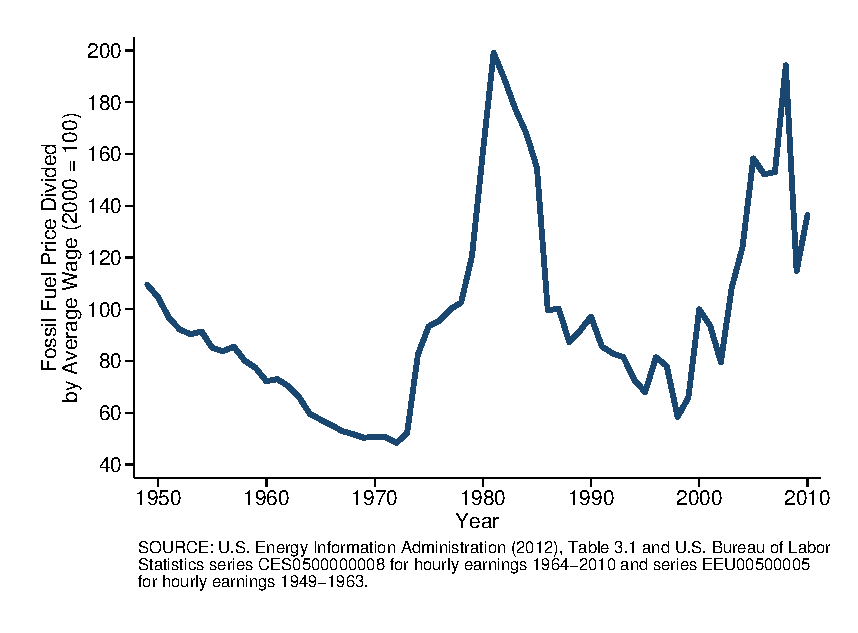
\includegraphics[scale=1.2]{figure_10_2.eps}
\end{center}
}

\slide{Commodity Prices and Wages}{Definitive downward trend
\begin{center}
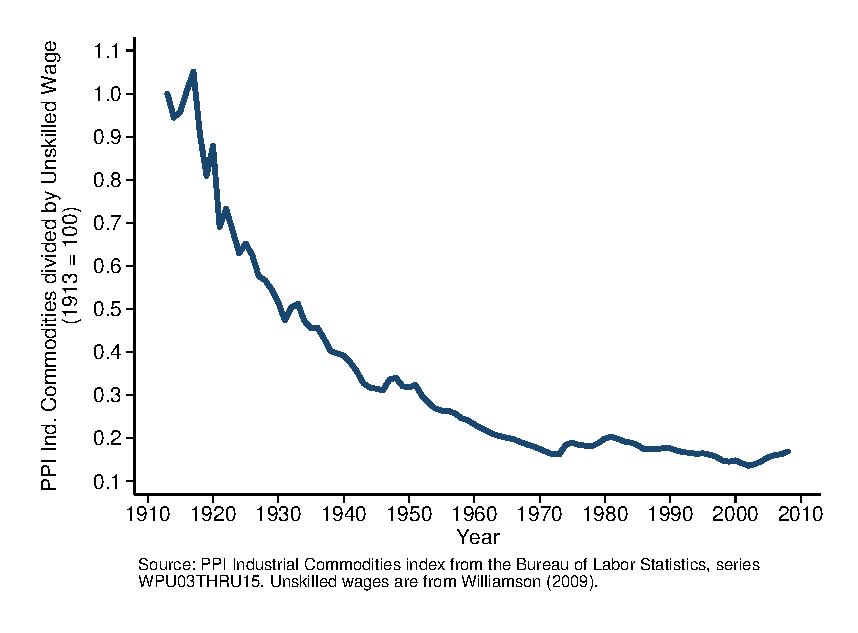
\includegraphics[scale=1.2]{figure_10_3.eps}
\end{center}
}

\slide{Fossil Fuel's Factor Share $v_E$}{No upward trend - maybe constant?
\begin{center}
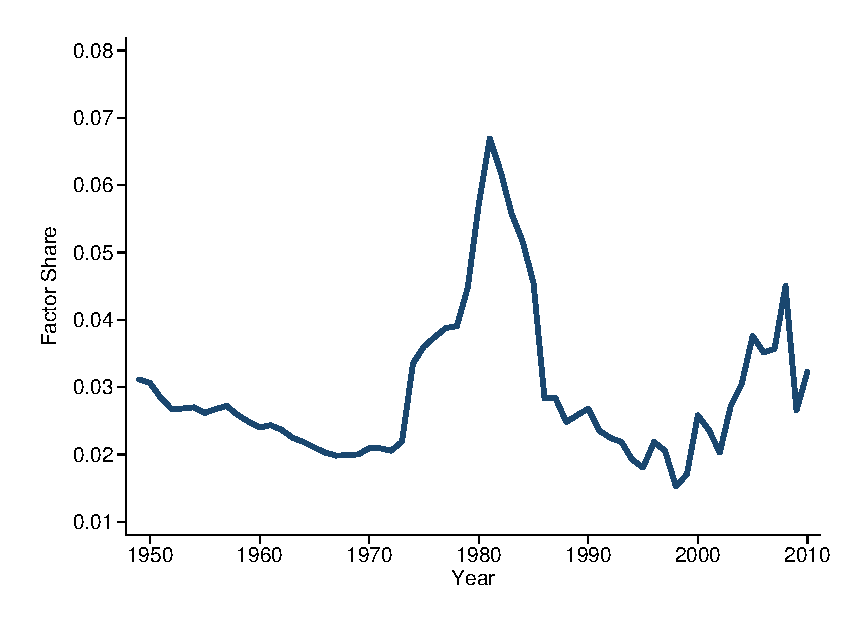
\includegraphics[scale=1.2]{figure_10_4.eps}
\end{center}
}

\slide{Energy Use per Person, $E/L$}{No tendency for $E/L$ to fall over time, actually rises
\begin{center}
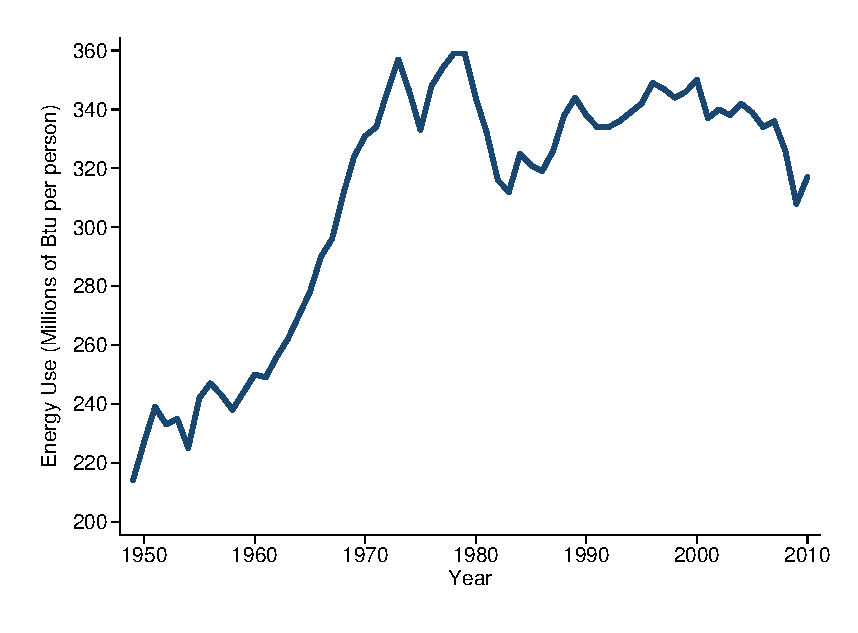
\includegraphics[scale=1.2]{figure_10_5.eps}
\end{center}
}

\slide{Factor Shares Changing}{We don't see massive price increases in resources, as $E/L$ is not falling, and $v_E$ seems to decline somewhat. 

\vspace{.25in}\noindent Want to be a little more nuanced about factor shares. Let
\begin{equation}
Y = (K^{\rho} + (BE)^{\rho})^{1/\rho}
\end{equation}
where we ignore labor for now to keep things simple.

\vspace{.25in}\noindent This is \textit{constant elasticity of substitution} function. $1/(1-\rho)$ is how EOS between capital and energy. $B$ is energy productivity.
\begin{itemize}
	\item If $0<\rho<1$, then $1/(1-\rho)>1$ and substitute capital for energy easily (or v.v.)
	\item If $\rho<1$, then $1/(1-\rho)<1$ and cannot substitute capital for energy easily (or v.v.)
\end{itemize}

\vspace{.25in}\noindent Energy's share of output with this function is
\begin{equation}
v_E = \left( \frac{BE}{Y}  \right)^{\rho}
\end{equation}
}

\slide{Energy's Share}{Using
\begin{equation}
v_E = \left( \frac{BE}{Y}  \right)^{\rho}
\end{equation}
what do we expect to happen to energy's share of output? We have, and expect that $E/Y$ is declining over time - value in 2010 about half of that in 1950 (Annual Energy Report, U.S. Energy Department). 

\vspace{.25in}\noindent Two ways for $v_E$ to decline given $E/Y$ is declining
\begin{itemize}
	\item If $\rho>0$, then as $E/Y$ falls, we substitute towards $K$, and energy isn't used as much. Energy isn't necessary for production. 
	\item If $\rho<0$, then as $E/Y$ falls, we cannot subsitute towards $K$, energy is vital to production.
\end{itemize}

\vspace{.25in}\noindent Seems likely that $\rho<0$, we need energy to produce. So only option left is that $B$ must be rising very quickly to drive down $v_E$ (or keep it from rising).

\vspace{.25in}\noindent We appear to be able to innovate away from using resources (e.g. fiber optics for copper) fast enough to avoid rapidly rising resource prices. In the future: ????????
}

\slide{Growth and the Environment}{Have not considered resources as anything other than inputs to production at this point. What if we value environmental quality, and resource extraction makes that worse?

\vspace{.25in}\noindent Let utility be
\begin{equation}
V = u(C_t) + \rho v(R_{t+1})
\end{equation}
where $C_t$ is how much we consume, and $R_{t+1}$ is the stock of remaining resources. 
\begin{itemize}
	\item $u(C_t)$ is utility from consumption, and we assume that it has diminishing marginal utility, or $u'(C_t)$ falls as we consume more
	\item $v(R_{t+1})$ is utility from the stock of resources left (e.g. untapped Artic wildlife preserves), and it also has diminishing marginal utility. Means that as the stock of resources \textit{falls}, marginal utility gets \textit{higher}.
\end{itemize}

\vspace{.25in}\noindent Question will be how to pick $C$ and $R_{t+1}$ to maximize utility.

}

\slide{Resources and Consumption}{Production is
\begin{equation}
C_t = B E_t^{\gamma} L_Y^{1-\gamma}
\end{equation}
and
\begin{equation}
R_{t+1} = R_t - E_t
\end{equation}
So using $E_t$ to increase consumption means we have a smaller stock of $R_{t+1}$ left over to enjoy. There's a trade-off in using resources. 

\vspace{.25in}\noindent Using discrete time, $R_{t+1}$ for simplicity.
}

\slide{Optimization}{Optimal use of resources. Take derivative of utility with respect to $E_t$, 
\begin{equation}
u'(C_t)\frac{\partial C_t}{\partial E_t} + \rho v'(R_{t+1})\frac{\partial R_{t+1}}{\partial E_t} = 0
\end{equation}
Evaluate the two partial derivatives
\begin{equation}
\frac{\partial C_t}{\partial E_t} = \gamma B E_t^{\gamma - 1} L_Y^{1-\gamma} = \gamma \frac{Y_t}{E_t}
\end{equation}
which comes from the production function, and 
\begin{equation}
\frac{\partial R_{t+1}}{\partial E_t} = -1
\end{equation}
which comes from the resource equation.

\vspace{.25in}\noindent Put those partials into the FOC at the top to get 
\begin{equation}
\frac{E_t}{Y_t} = \frac{\gamma}{\rho} \frac{u'(C_t)}{v'(R_{t+1})}
\end{equation}
}

\slide{Environment and Growth}{Given the relationship
\begin{equation}
\frac{E_t}{Y_t} = \frac{\gamma}{\rho} \frac{u'(C_t)}{v'(R_{t+1})}
\end{equation}
\begin{itemize}
	\item As consumption, $C_t$, gets high, the marginal utility of consumption, $u'(C_t)$, falls. 
	\item As we use up resources, $R_{t+1}$ gets small, and the marginal utility, $v'(R_{t+1})$, gets big.
	\item Both these forces suggest that the ratio of $E_t/Y_t$ should \textit{fall} as countries get richer
	\item For very poor countries, the ratio of $E_t/Y_t$ may \textit{rise} as they get richer, because the marginal utility of resources may be negligible and the MU of consumption remains high
\end{itemize}

}

\slide{Pollution and Growth}{Implies falling pollution (better environment) as we get richer
\begin{center}
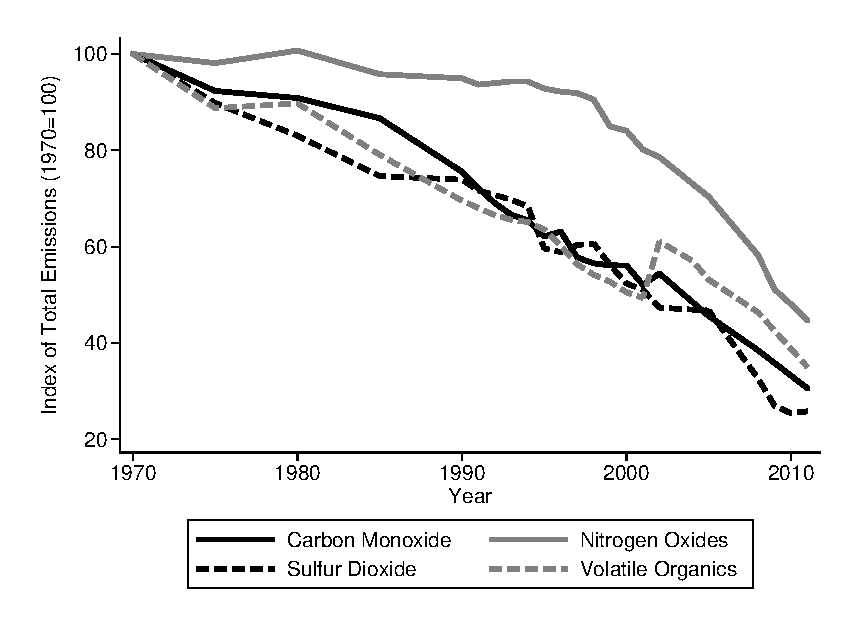
\includegraphics[scale=1.2]{figure_10_6.eps}
\end{center}
}

\slide{Factors in Changing Environmentalism}{Consider several ways of thinking about environment/growth link
\begin{itemize}
	\item $L_Y$ are production workers. $L_Y$ may fall if we allocate more people to solving environmental issues, or cleaning up environment, or simply idling them if we want to avoid pollution
	\item $\gamma$ is importance of energy in production. One aspect of innovation is lowering $\gamma$, which would naturally reduce environmental impact (e.g. solar)
	\item $\rho$ is our concern for the environment in the future. As we live longer, we may put more weight on utility from $R_{t+1}$ compared to consumption today, lowering our willingness to use energy/resources.
\end{itemize}

\vspace{.25in}\noindent Is there a ``right'' value for $\rho$? Nothing this problem can say about that. People speculate/argue over it. What is right weight to put on future generations having access to $R_{t+1}$?
}

\end{document}